%\documentclass[12pt,a4paper]{article}
%\usepackage{amsmath,amssymb,amsthm}
%\usepackage{geometry}

%\usepackage{changepage}

%\usepackage{xltxtra,fontspec,xunicode}
%\defaultfontfeatures{Scale=MatchLowercase,Mapping=tex-text}

%\usepackage{parskip}

%\begin{document}
\setlength\parindent{0pt}

%\section*{Appendix B: Experimental instructions}



\subsection*{Instructions for the experiment}
\emph{<Presented as a pdf document and available throughout the experiment>}
\bigskip

\textbf{These instructions are identical to all the participants.}

\textbf{The experiment is composed of five separate and different phases.} At the beginning of the experiment, all participants will be allocated into \textbf{teams of four}. Each team has a unique \textbf{colour}. These teams will remain fixed throughout the experiment.

Before each part, we will distribute and read the relevant instructions for that part. In each part the participants will be reallocated into groups. The number of participants in a group can change from part to part. The payments in the part will be determined according to the decisions of the participants in the team. It is possible, but not necessary, that another participant will be in the same group as you in two different parts. In each part of the experiment you will be able to know which team each of the participants in your group belongs to.

\textbf{Your final payment in the experiment will be the total of your gain in all of the parts}.

At the end of the experiment, you will be presented with the payments in each part and your total payment, in points and in shekels. Please remain seated until the experimenter calls you for payment.

\textbf{If you have any questions, please raise your hand now and the experimenter will come to you}.

\newpage

\subsection*{Experiments for the first part}

In this part, you and the members of your team perform a pattern completion task. The computer will present you with five questions. Each question is comprised of eight pictures, and the team members wil be asked to choose a ninth picture out of eight possible pictures to complete the pattern. For example:

\begin{center}
	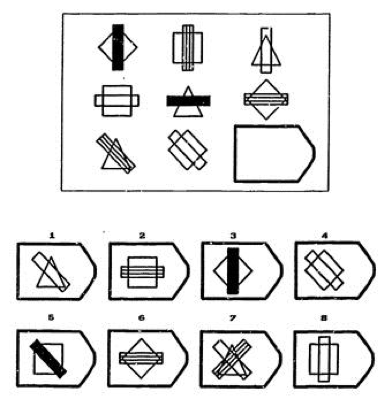
\includegraphics[]{Raven.png}
\end{center}

Each team member must answer all of the questions. For each correct answer, the team member will receive \textbf{10 points}. Additionally, if all of the team members answer correctly, the whole team will receive a \textbf{team bonus of 20 points, to be equally divided among the team members}.

\textbf{Each question will be allocated two minutes}. During this time, the team members can \textbf{consult each other} using electronic chat. Enter your answer and click Confirm. You can change your answer and click Confirm again at any point during the two minutes. The last answer to be entered is the final answer.

\textbf{Attention:} Do not reveal any identifying information. If any participant in the session identifies themselves, we will stop the experiment and release all participants with only the showup fee.

\textbf{If you have any questions, please raise your hand now and the experimenter will come to you}.

\newpage

\subsection*{Instructions for the second part}

In this part participants will be matched in \textbf{pairs}. In each pair, one participant will be in role A and the other participant in role B. Participant A receives an allocation of \textbf{150 points} and decides how many of the 150 points to \textbf{send to Participant B}. The amount is \textbf{tripled}. Next, Participant B will decide how many points out of the points received to \textbf{send back to to Participant A}. These points will not be multiplied.

If you are allocated to role A, your payment in this part will be:

\newcommand{\boxit}[2]{\fbox{\begin{minipage}[c][4cm][c]{#1}\centering #2\end{minipage}}}
\setlength\fboxrule{3pt}

{\medskip%\hspace{-2cm}
\begin{adjustwidth}{-0.6in}{-0.6in}
\large
\sffamily\centering
\boxit{1.5cm}{\Huge 150} -
\boxit{4cm}{The number of points you sent to Participant B} +
\boxit{4cm}{\large The number of points Participant B sent back} =
\boxit{2cm}{Second part earnings}
\end{adjustwidth}
}\medskip

If you are allocated to role B, your payment in this part will be:

{\medskip%\hspace{-2cm}
\begin{adjustwidth}{-0.6in}{-0.6in}
\large
\sffamily\centering
\boxit{1.5cm}{\Huge 3} $\times$
\boxit{4cm}{The number of points Participant A sent you} -
\boxit{4cm}{\large The number of points you sent back} =
\boxit{2cm}{Second part earnings}
\end{adjustwidth}
}\medskip

Before making your decision, you will be able to test the payment calculation in a \textbf{practice phase}, in which you will be able to make decisions as both \textbf{Participant A} and as \textbf{Participant B}. In this stage, you will enter decisions in both roles, and see the final payments. The practice will repeat five times. 

\textbf{If you have any questions, please raise your hand now and the experimenter will come to you}.

\newpage

\subsection*{Instructions for the third part}

In the third part, all participants will be matched in \textbf{groups of three}. Each of the three participants in the group will choose how to \textbf{divide 100 points} between the three group members, such that he himself receives \textbf{30 points}, and \textbf{freely allocates} the remaining \textbf{70 points} between the other two group members. This stage has \textbf{6 rounds}, and you will be \textbf{rematched in a new group}.

\subsection*{Payment calculation in the part}

At the end of the experiment, the computer will randomly choose one of the six rounds, and one participant in each group. The payment for this part will be determined according to the decision of the randomly chosen participant in the randomly chosen round.

\textbf{If you have any questions, please raise your hand now and the experimenter will come to you}.

\newpage

\subsection*{Instructions for the fourth part}

In this part, participant will be matched in \textbf{pairs}. 

Each participant will be presented with \textbf{6 rulers} that include nine possible allocations of money to the two participants. The amount you chose to \textbf{keep for yourself} is indicated above each ruler, and the amount you choose to \textbf{give to the other participant} is indicated below the ruler. You are to choose your preferred allocation of the nine possible allocations. For example, 
\smallskip

\begin{center}
	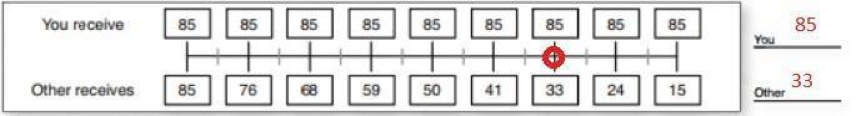
\includegraphics[]{svo.png}
\end{center}

You can choose any point on the ruler. For example, assume you chose the point marked in red. You will receive 85 points and the other participant will receive 33 points.

At the end of the part, the computer will randomly choose on of the two participants in the pair and one of the nine rulers. your payment in this part will be determined by the decision of the randomly chosen participant for the randomly chosen ruler.

\textbf{If you have any questions, please raise your hand now and the experimenter will come to you}.

\newpage

\subsection*{Instructions for the fifth part}

In this part you will be asked to answer several questions. The questions have to do with the way one sees himself and his surroundings in different situations. Your task is to indicate how much you agree or disagree with each statement, using the following scale:
\begin{enumerate}
	\item Strongly disagree.
	\item Disagree.
	\item Neither agree nor disagree.
	\item Agree.
	\item Strongly agree.
\end{enumerate}

Note: there are no right and wrong answers. Please indicate the answer that best reflects your character with respect to the statement. Take your time and think about your answer.


%\end{document} 